\documentclass[aspectratio=169,12pt]{beamer}
\usepackage{amsmath}
\usepackage{amssymb}
\usepackage{xcolor}
\usepackage[most]{tcolorbox}
\usepackage{tikz}
\usepackage{graphicx}
\usepackage[sfdefault,lf]{FiraSans}
\renewcommand{\familydefault}{\sfdefault}
\setlength{\parindent}{0pt}
\setbeamertemplate{navigation symbols}{}
\setbeamertemplate{footline}{}
\setbeamertemplate{headline}{}
\definecolor{mmpageWhite}{HTML}{FCFBF7}
\definecolor{mmtanSoft}{HTML}{F7F5EF}
\definecolor{mmgreenDeep}{HTML}{244B2C}
\definecolor{mmgreenLeaf}{HTML}{5D8A56}
\definecolor{mmtext}{HTML}{163221}
\definecolor{mmanswerColor}{HTML}{306A3A}
\setbeamercolor{background canvas}{bg=mmpageWhite}
\setbeamercolor{normal text}{fg=mmtext,bg=mmpageWhite}
\newtcolorbox{AnsCard}[1][]{enhanced,breakable=false,colback=white,colframe=black,boxrule=1.5pt,arc=8pt,left=5pt,right=5pt,top=4pt,bottom=4pt,before skip=0pt,after skip=0pt,height=0.4\textheight,valign=center,#1}
\newcommand{\KoruIcon}{\raisebox{-0.2em}{
\includegraphics[height=1.05em]{img/header-logo.png}}}
\newcommand{\HoeIcon}{\raisebox{-0.2em}{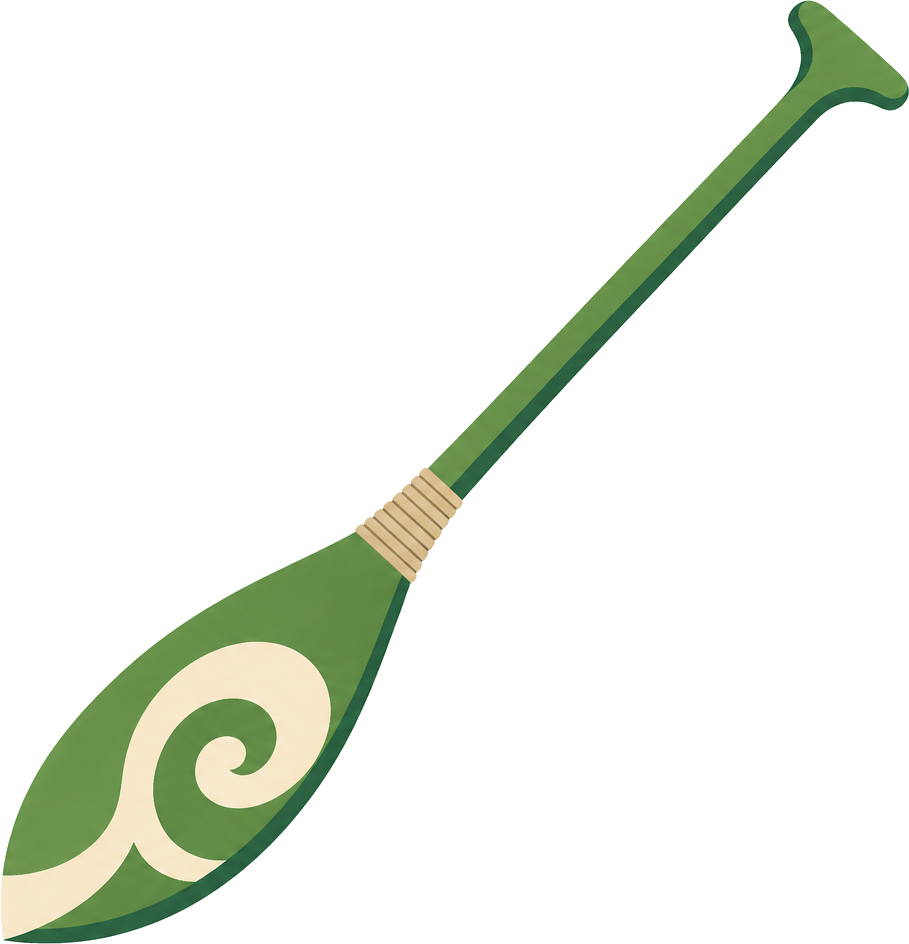
\includegraphics[height=1.05em]{img/hoe.png}}}
\newcommand{\ScaffoldIcons}[1]{\ifcase#1\or \HoeIcon\or \HoeIcon\hspace{0.22em}\HoeIcon\or \HoeIcon\hspace{0.22em}\HoeIcon\hspace{0.22em}\HoeIcon\fi}
\newcommand{\WorksheetTitle}[2]{%
  {\colorbox{mmtanSoft}{\parbox[c][2.2em][c]{0.975\linewidth}{%
    \hspace{0.25em}{\Large\bfseries\textcolor{mmgreenDeep}{#1}\hfill\ScaffoldIcons{#2}}}}
  \par\vspace{0.12em}{\color{mmgreenLeaf}\rule{\linewidth}{2.5pt}}\par\vspace{0.06em}}
}
\setbeamertemplate{background}{
 \begin{tikzpicture}[remember picture,overlay]
 \draw[black,line width=1.5pt,rounded corners=10pt]
 ([xshift=0.45cm,yshift=-0.45cm]current page.north west)
 rectangle
 ([xshift=-0.45cm,yshift=0.45cm]current page.south east);
 \end{tikzpicture}
}
\begin{document}
\begin{frame}[t]
\WorksheetTitle{Start Tasks - Answers}{1}
\vspace{-0.1em}
\begin{columns}[T,onlytextwidth]
\begin{column}{0.48\textwidth}\begin{AnsCard}\small\textcolor{mmgreenDeep}{\textbf{1. Cube side 4 cm}}\\\vspace{0.1em}\textcolor{mmanswerColor}{\textbf{SA = 6(4$^2$) = 6(16) = 96 cm$^2$}}\end{AnsCard}\end{column}
\begin{column}{0.48\textwidth}\begin{AnsCard}\small\textcolor{mmgreenDeep}{\textbf{2. Cube side 7 m}}\\\vspace{0.1em}\textcolor{mmanswerColor}{\textbf{SA = 6(7$^2$) = 6(49) = 294 m$^2$}}\end{AnsCard}\end{column}
\end{columns}
\vspace{0.15em}
\begin{columns}[T,onlytextwidth]
\begin{column}{0.48\textwidth}\begin{AnsCard}\small\textcolor{mmgreenDeep}{\textbf{3. Cuboid 8$\times$3$\times$2 cm}}\\\vspace{0.1em}\textcolor{mmanswerColor}{\textbf{SA = 2(8$\cdot$3+8$\cdot$2+3$\cdot$2) = 2(46) = 92 cm$^2$}}\end{AnsCard}\end{column}
\begin{column}{0.48\textwidth}\begin{AnsCard}\small\textcolor{mmgreenDeep}{\textbf{4. Cuboid 10$\times$4$\times$2 m}}\\\vspace{0.1em}\textcolor{mmanswerColor}{\textbf{SA = 2(10$\cdot$4+10$\cdot$2+4$\cdot$2) = 2(68) = 136 m$^2$}}\end{AnsCard}\end{column}
\end{columns}
\vspace{0.15em}
\begin{columns}[T,onlytextwidth]
\begin{column}{0.48\textwidth}\begin{AnsCard}\small\textcolor{mmgreenDeep}{\textbf{5. One face of cube side 6 cm}}\\\vspace{0.1em}\textcolor{mmanswerColor}{\textbf{A = 6$^2$ = 36 cm$^2$}}\end{AnsCard}\end{column}
\begin{column}{0.48\textwidth}\begin{AnsCard}\small\textcolor{mmgreenDeep}{\textbf{6. Cube one face 25 cm$^2$}}\\\vspace{0.1em}\textcolor{mmanswerColor}{\textbf{SA = 6 $\times$ 25 = 150 cm$^2$}}\end{AnsCard}\end{column}
\end{columns}
\end{frame}
\begin{frame}[t]
\WorksheetTitle{Start Tasks - Answers}{1}
\vspace{-0.1em}
\begin{columns}[T,onlytextwidth]
\begin{column}{0.48\textwidth}\begin{AnsCard}\small\textcolor{mmgreenDeep}{\textbf{7. Top+bottom of 9$\times$5$\times$4}}\\\vspace{0.1em}\textcolor{mmanswerColor}{\textbf{2(9 $\times$ 5) = 2(45) = 90 cm$^2$}}\end{AnsCard}\end{column}
\begin{column}{0.48\textwidth}\begin{AnsCard}\small\textcolor{mmgreenDeep}{\textbf{8. Four side faces}}\\\vspace{0.1em}\textcolor{mmanswerColor}{\textbf{2(9$\times$4)+2(5$\times$4) = 72+40 = 112 cm$^2$}}\end{AnsCard}\end{column}
\end{columns}
\vspace{0.15em}
\begin{columns}[T,onlytextwidth]
\begin{column}{0.48\textwidth}\begin{AnsCard}\small\textcolor{mmgreenDeep}{\textbf{9. Gift box 12$\times$5$\times$3 cm}}\\\vspace{0.1em}\textcolor{mmanswerColor}{\textbf{SA = 2(60+36+15) = 2(111) = 222 cm$^2$}}\end{AnsCard}\end{column}
\begin{column}{0.48\textwidth}\begin{AnsCard}\small\textcolor{mmgreenDeep}{\textbf{10. Fish tank (no lid)}}\\\vspace{0.1em}\textcolor{mmanswerColor}{\textbf{Base+sides: 1000+3900 = 4900 cm$^2$}}\end{AnsCard}\end{column}
\end{columns}
\vspace{0.15em}
\begin{columns}[T,onlytextwidth]
\begin{column}{0.48\textwidth}\begin{AnsCard}\small\textcolor{mmgreenDeep}{\textbf{11. Cube SA = 54, find side}}\\\vspace{0.1em}\textcolor{mmanswerColor}{\textbf{6s$^2$ = 54 $\to$ s$^2$ = 9 $\to$ s = 3 cm}}\end{AnsCard}\end{column}
\begin{column}{0.48\textwidth}\begin{AnsCard}\small\textcolor{mmgreenDeep}{\textbf{12. Greatest face pair}}\\\vspace{0.1em}\textcolor{mmanswerColor}{\textbf{6 $\times$ 4 = 24 cm$^2$ (largest)}}\end{AnsCard}\end{column}
\end{columns}
\end{frame}
\begin{frame}[t]
\WorksheetTitle{Start Tasks - Answers}{1}
\vspace{-0.1em}
\begin{columns}[T,onlytextwidth]
\begin{column}{0.48\textwidth}\begin{AnsCard}\small\textcolor{mmgreenDeep}{\textbf{13. Top/bottom total 96 cm$^2$}}\\\vspace{0.1em}\textcolor{mmanswerColor}{\textbf{2(8$\times$6) = 96, consistent}}\end{AnsCard}\end{column}
\begin{column}{0.48\textwidth}\begin{AnsCard}\small\textcolor{mmgreenDeep}{\textbf{14. Why square units?}}\\\vspace{0.1em}\textcolor{mmanswerColor}{\textbf{SA is 2D area, so cm$^2$ not cm$^3$}}\end{AnsCard}\end{column}
\end{columns}
\vspace{0.15em}
\begin{columns}[T,onlytextwidth]
\begin{column}{0.48\textwidth}\begin{AnsCard}\small\textcolor{mmgreenDeep}{\textbf{15. Cube 0.5 m}}\\\vspace{0.1em}\textcolor{mmanswerColor}{\textbf{SA = 6(0.5$^2$) = 6(0.25) = 1.5 m$^2$}}\end{AnsCard}\end{column}
\begin{column}{0.48\textwidth}\begin{AnsCard}\small\textcolor{mmgreenDeep}{\textbf{16. Cuboid 7$\times$2$\times$5}}\\\vspace{0.1em}\textcolor{mmanswerColor}{\textbf{SA = 2(14+35+10) = 2(59) = 118 cm$^2$}}\end{AnsCard}\end{column}
\end{columns}
\vspace{0.15em}
\begin{columns}[T,onlytextwidth]
\begin{column}{0.48\textwidth}\begin{AnsCard}\small\textcolor{mmgreenDeep}{\textbf{17. Die side 1.5 cm}}\\\vspace{0.1em}\textcolor{mmanswerColor}{\textbf{SA = 6(1.5$^2$) = 6(2.25) = 13.5 cm$^2$}}\end{AnsCard}\end{column}
\begin{column}{0.48\textwidth}\begin{AnsCard}\small\textcolor{mmgreenDeep}{\textbf{18. Square prism 3$\times$3$\times$10}}\\\vspace{0.1em}\textcolor{mmanswerColor}{\textbf{2(9)+4(30) = 18+120 = 138 cm$^2$}}\end{AnsCard}\end{column}
\end{columns}
\end{frame}
\end{document}
